
%! Tex program = xelatex
\documentclass[UTF8]{article}
\usepackage{indentfirst}
\usepackage{graphicx} 
\usepackage{amsmath}  
\usepackage{float}   
\usepackage{listings}

\title{Discrete Mathematics}
\author{Zhengren Wang 2019081308021}
\date{06/02/2020 Tue}
\begin{document}
\maketitle 
\part{10.1}
\begin{description}
    \item[11]Let $G$ be a simple graph. Show that the relation $R$ on the set of vertices of $G$ such that $uRv$ if and only if there is an edge associated to $\{u, v\}$ is a symmetric, irreflexive relation on $G$.  \\\\
        Symmetric: $\forall uRv$, there will be an edge associated with \{u, v\}. and \{u, v\}=\{v, u\}, so this edge is associated with \{v, u\} and therefore $vRu$. Thus, $R$ is a symmetric relation.  \\
        Irreflexive: In any simple graph, there is no loop. So, \{u,u\} will not appear. Therefore, $uRu$ will not appear,so $R$ is irreflexive.
    \item[13]The intersection graph of a collection of sets $A_1, A_2,\cdots,A_n$ is the graph that has a vertex for each of these sets and has an edge connecting the vertices representing two sets if these sets have a nonempty intersection. Construct the intersection graph of these collections of sets.

            a) A1 = $\{0, 2, 4, 6, 8\}$ \\
               A2 = $\{0, 1, 2, 3, 4\}$ \\
               A3 = $\{1, 3, 5, 7, 9\}$ \\
               A4 = $\{5, 6, 7, 8, 9\}$ \\
               A5 = $\{0, 1, 8, 9\}$    \\

            b) A1 = $\{..., −4, −3, −2, −1, 0\}$          \\
               A2 = $\{..., −2, −1, 0, 1, 2,...\}$        \\
               A3 = $\{..., −6, −4, −2, 0, 2, 4, 6,...\}$ \\
               A4 = $\{..., −5, −3, −1, 1, 3, 5,...\}$    \\
               A5 = $\{..., −6, −3, 0, 3, 6,...\}$         \\

            c) A1 = $\{x | x < 0\}$    \\
               A2 = $\{x | −1 <x< 0\}$ \\
               A3 = $\{x | 0 <x< 1\}$  \\
               A4 = $\{x | −1 <x< 1\}$ \\
               A5 = $\{x | x > −1\}$   \\
               A6 = $R$               \\
            \\ 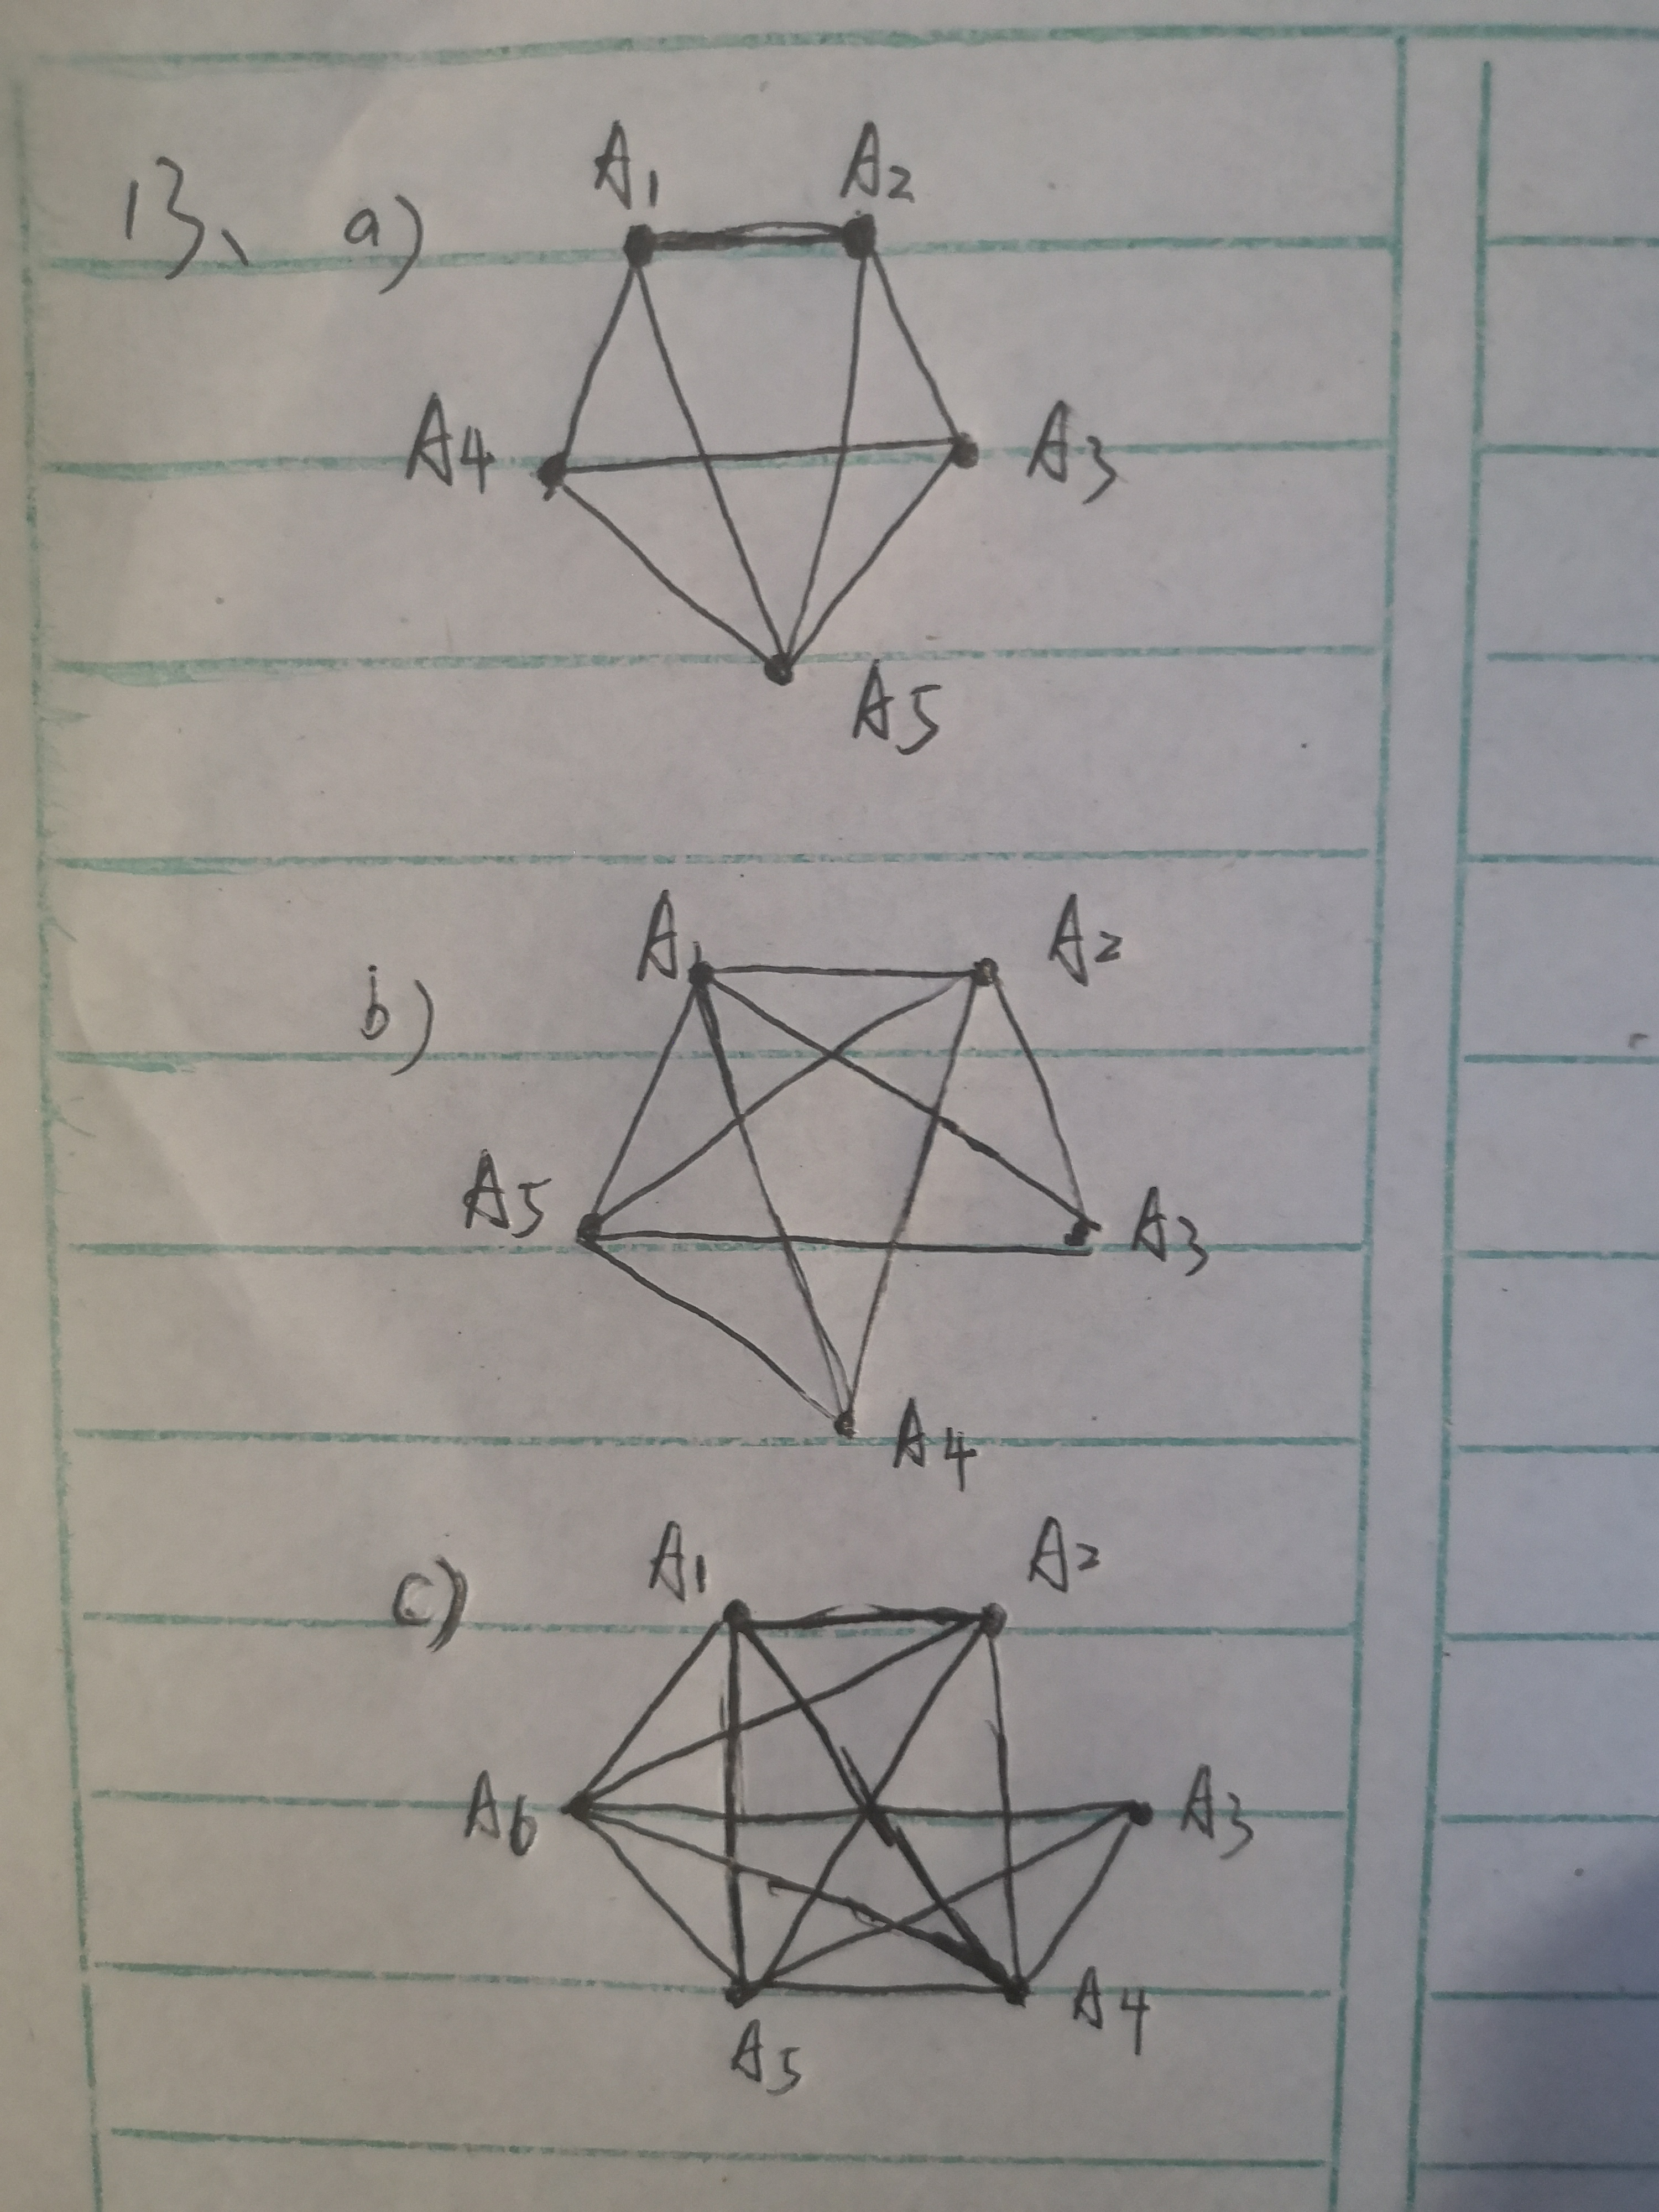
\includegraphics[scale=0.1]{../imgs/10_1_13.jpg}  \\ 

\end{description}

\end{document}
